%% abtex2-modelo-artigo.tex, v-1.9.7 laurocesar
%% Copyright 2012-2018 by abnTeX2 group at http://www.abntex.net.br/ 
%%
%% This work may be distributed and/or modified under the
%% conditions of the LaTeX Project Public License, either version 1.3
%% of this license or (at your option) any later version.
%% The latest version of this license is in
%%   http://www.latex-project.org/lppl.txt
%% and version 1.3 or later is part of all distributions of LaTeX
%% version 2005/12/01 or later.
%%
%% This work has the LPPL maintenance status `maintained'.
%% 
%% The Current Maintainer of this work is the abnTeX2 team, led
%% by Lauro César Araujo. Further information are available on 
%% http://www.abntex.net.br/
%%
%% This work consists of the files abntex2-modelo-artigo.tex and
%% abntex2-modelo-references.bib
%%

% ------------------------------------------------------------------------
% ------------------------------------------------------------------------
% abnTeX2: Modelo de Artigo Acadêmico em conformidade com
% ABNT NBR 6022:2018: Informação e documentação - Artigo em publicação 
% periódica científica - Apresentação
% ------------------------------------------------------------------------
% ------------------------------------------------------------------------

\documentclass[
% -- opções da classe memoir --
article,			% indica que é um artigo acadêmico
11pt,				% tamanho da fonte
oneside,			% para impressão apenas no recto. Oposto a twoside
a4paper,			% tamanho do papel. 
% -- opções da classe abntex2 --
%chapter=TITLE,		% títulos de capítulos convertidos em letras maiúsculas
%section=TITLE,		% títulos de seções convertidos em letras maiúsculas
%subsection=TITLE,	% títulos de subseções convertidos em letras maiúsculas
%subsubsection=TITLE % títulos de subsubseções convertidos em letras maiúsculas
% -- opções do pacote babel --
english,			% idioma adicional para hifenização
brazil,				% o último idioma é o principal do documento
sumario=tradicional
]{abntex2}


% ---
% PACOTES
% ---

% ---
% Pacotes fundamentais 
% ---
\usepackage{lmodern}			% Usa a fonte Latin Modern
\usepackage[T1]{fontenc}		% Selecao de codigos de fonte.
\usepackage[utf8]{inputenc}		% Codificacao do documento (conversão automática dos acentos)
\usepackage{indentfirst}		% Indenta o primeiro parágrafo de cada seção.
\usepackage{nomencl} 			% Lista de simbolos
\usepackage{color}				% Controle das cores
\usepackage{graphicx}			% Inclusão de gráficos
\usepackage{microtype} 			% para melhorias de justificação
% ---

% ---
% Pacotes adicionais, usados apenas no âmbito do Modelo Canônico do abnteX2
% ---
\usepackage{lipsum}				% para geração de dummy text
% ---

% ---
% Pacotes de citações
% ---
\usepackage[brazilian,hyperpageref]{backref}	 % Paginas com as citações na bibl
\usepackage[alf]{abntex2cite}	% Citações padrão ABNT
% ---

% ---
% Configurações do pacote backref
% Usado sem a opção hyperpageref de backref
\renewcommand{\backrefpagesname}{Citado na(s) página(s):~}
% Texto padrão antes do número das páginas
\renewcommand{\backref}{}
% Define os textos da citação
\renewcommand*{\backrefalt}[4]{
	\ifcase #1 %
	Nenhuma citação no texto.%
	\or
	Citado na página #2.%
	\else
	Citado #1 vezes nas páginas #2.%
	\fi}%
% ---

% --- Informações de dados para CAPA e FOLHA DE ROSTO ---
\titulo{Tutorial de Desenvolvimento com FrameWeb SPA}
\tituloestrangeiro{FrameWeb SPA Development Tutorial}

\autor{
	Pedro Henrique Brunoro Hoppe\thanks{``Mestrando.'' \url{pedrohoppe@gmail.com}} 
	\\[0.5cm] 
	Vitór Estêvao Silva Souza\thanks{``Constar currículo sucinto de cada autor, com 
		vinculação corporativa e endereço de contato.''} }

\local{Brasil}
\data{2022}
% ---

% ---
% Configurações de aparência do PDF final

% alterando o aspecto da cor azul
\definecolor{blue}{RGB}{41,5,195}

% informações do PDF
\makeatletter
\hypersetup{
	%pagebackref=true,
	pdftitle={\@title}, 
	pdfauthor={\@author},
	pdfsubject={Modelo de artigo científico com abnTeX2},
	pdfcreator={LaTeX with abnTeX2},
	pdfkeywords={abnt}{latex}{abntex}{abntex2}{atigo científico}, 
	colorlinks=true,       		% false: boxed links; true: colored links
	linkcolor=blue,          	% color of internal links
	citecolor=blue,        		% color of links to bibliography
	filecolor=magenta,      		% color of file links
	urlcolor=blue,
	bookmarksdepth=4
}
\makeatother
% --- 

% ---
% compila o indice
% ---
\makeindex
% ---

% ---
% Altera as margens padrões
% ---
\setlrmarginsandblock{3cm}{3cm}{*}
\setulmarginsandblock{3cm}{3cm}{*}
\checkandfixthelayout
% ---

% --- 
% Espaçamentos entre linhas e parágrafos 
% --- 

% O tamanho do parágrafo é dado por:
\setlength{\parindent}{1.3cm}

% Controle do espaçamento entre um parágrafo e outro:
\setlength{\parskip}{0.2cm}  % tente também \onelineskip

% Espaçamento simples
\SingleSpacing


% ----
% Início do documento
% ----
\begin{document}
	
	% Seleciona o idioma do documento (conforme pacotes do babel)
	%\selectlanguage{english}
	\selectlanguage{brazil}
	
	% Retira espaço extra obsoleto entre as frases.
	\frenchspacing 
	
	% ----------------------------------------------------------
	% ELEMENTOS PRÉ-TEXTUAIS
	% ----------------------------------------------------------
	
	%---
	%
	% Se desejar escrever o artigo em duas colunas, descomente a linha abaixo
	% e a linha com o texto ``FIM DE ARTIGO EM DUAS COLUNAS''.
	% \twocolumn[    		% INICIO DE ARTIGO EM DUAS COLUNAS
	%
	%---
	
	% página de titulo principal (obrigatório)
	\maketitle
	
	
	% titulo em outro idioma (opcional)
	
	% ----------------------------------------------------------
	% ELEMENTOS TEXTUAIS
	% ----------------------------------------------------------
	\textual
	
	% ----------------------------------------------------------
	% Introdução
	% ----------------------------------------------------------
\section{Instalação}
	
\subsection{Instalação do FrameWeb SPA}
Para instalar o FrameWeb SPA acesse o sítio eletrônico \url{https://github.com/pedrohbh/FrameWebSPA} e clone o repositório para sua máquina (ou baixe o zip disponível em ``Code'' -> ``Download Zip'') [\autoref{fig:tutorial-1}].

\begin{figure}
	\centering
	\includegraphics[width=\linewidth]{"figuras/Tutorial 1"}
	\caption{Repositório GitHub}
	\label{fig:tutorial-1}
\end{figure}

Após baixar o repositório, siga os seguintes passos:
\begin{enumerate}
	\item Abra o Eclipse;
	\item Clique no menu Help -> Install New Software...;
	\item Clique em ``Add...'' (\autoref{fig:siriustuto516});
	\item Preencha os campos:
	\begin{description}
		\item[Name:] Pode ser o nome que você quiser. \textit{Sugestão: FrameWeb SPA};
		\item[Location:] Clique no botão ``Archive…'' e depois selecione o arquivo ``FrameWeb.zip'' na pasta onde foi clonado o repositório do GitHub anteriormente;
	\end{description}
	\item Clique no botão ``Add'' (\autoref{fig:tutorial-2});
	\item Em ``Work with:'' selecione o repositório adicionado no passo anterior (no nosso caso, \textit{FrameWeb SPA}), marque as opções ``FrameWeb Code Generator'' e ``FrameWeb Graphical Editor'' e clique em ``Next >'' (\autoref{fig:tutorial-3});
	\item Siga os demais passos de instalação aceitando os termos de licença. Caso apareça uma mensagem dizendo que os certificados de segurança não são reconhecidos, apenas marque todos e clique em Ok;
	\item Após a instalação, reinicie o Eclipse.
\end{enumerate}

\begin{figure}
	\centering
	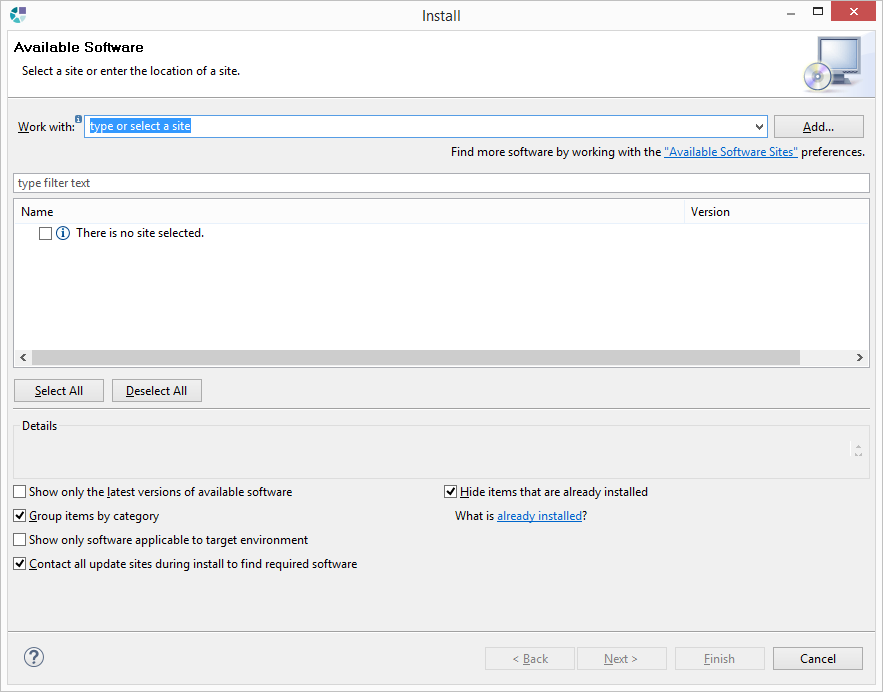
\includegraphics[width=0.7\linewidth]{figuras/Sirius_tuto5_16}
	\caption{Menu de instalação do Eclipse}
	\label{fig:siriustuto516}
\end{figure}

\begin{figure}
	\centering
	\includegraphics[width=0.7\linewidth]{"figuras/Tutorial 2"}
	\caption{Passo 5}
	\label{fig:tutorial-2}
\end{figure}

\begin{figure}
	\centering
	\includegraphics[width=0.7\linewidth]{"figuras/Tutorial 3"}
	\caption{Passo 6}
	\label{fig:tutorial-3}
\end{figure}



%Open Eclipse;
%Click on the menu Help > Install New Software...
%In the Work with: field, type http://dev.nemo.inf.ufes.br/framewebplugin/ and press Enter;
%Unmark the checkbox Group items by category;
%Mark the checkbox for all FrameWeb Tools that show in the list (see figure below);
%Click Next twice, select the I accept the terms of the license agreement option and then click Finish;
%After the installation, restart Eclipse.



\section{Desenvolvimento}
	
\subsection{Margens}
	
A norma ABNT NBR 6022:2018 não estabelece uma margem específica a ser utilizada
no artigo científico. Dessa maneira, caso deseje alterar as margens, utilize os
comandos abaixo:
	
\begin{verbatim}
	\setlrmarginsandblock{3cm}{3cm}{*}
	\setulmarginsandblock{3cm}{3cm}{*}
	\checkandfixthelayout
\end{verbatim}
	
\subsection{Duas colunas}
	
	É comum que artigos científicos sejam escritos em duas colunas. Para isso,
	adicione a opção \texttt{twocolumn} à classe do documento, como no exemplo:
	
	\begin{verbatim}
		\documentclass[article,11pt,oneside,a4paper,twocolumn]{abntex2}
	\end{verbatim}
	
	É possível indicar pontos do texto que se deseja manter em apenas uma coluna,
	geralmente o título e os resumos. Os resumos em única coluna em documentos com
	a opção \texttt{twocolumn} devem ser escritos no ambiente
	\texttt{resumoumacoluna}:
	
	\begin{verbatim}
		\twocolumn[              % INICIO DE ARTIGO EM DUAS COLUNAS
		
		\maketitle             % pagina de titulo
		
		\renewcommand{\resumoname}{Nome do resumo}
		\begin{resumoumacoluna}
			Texto do resumo.
			
			\vspace{\onelineskip}
			
			\noindent
			\textbf{Palavras-chave}: latex. abntex. editoração de texto.
		\end{resumoumacoluna}
		
		]                        % FIM DE ARTIGO EM DUAS COLUNAS
	\end{verbatim}
	
	\subsection{Recuo do ambiente \texttt{citacao}}
	
	Na produção de artigos (opção \texttt{article}), pode ser útil alterar o recuo
	do ambiente \texttt{citacao}. Nesse caso, utilize o comando:
	
	\begin{verbatim}
		\setlength{\ABNTEXcitacaorecuo}{1.8cm}
	\end{verbatim}
	
	Quando um documento é produzido com a opção \texttt{twocolumn}, a classe
	\textsf{abntex2} automaticamente altera o recuo padrão de 4 cm, definido pela
	ABNT NBR 10520:2002 seção 5.3, para 1.8 cm.
	
	\section{Cabeçalhos e rodapés customizados}
	
	Diferentes estilos de cabeçalhos e rodapés podem ser criados usando os
	recursos padrões do \textsf{memoir}.
	
	Um estilo próprio de cabeçalhos e rodapés pode ser diferente para páginas pares
	e ímpares. Observe que a diferenciação entre páginas pares e ímpares só é
	utilizada se a opção \texttt{twoside} da classe \textsf{abntex2} for utilizado.
	Caso contrário, apenas o cabeçalho padrão da página par (\emph{even}) é usado.
	
	Veja o exemplo abaixo cria um estilo chamado \texttt{meuestilo}. O código deve
	ser inserido no preâmbulo do documento.
	
	\begin{verbatim}
		%%criar um novo estilo de cabeçalhos e rodapés
		\makepagestyle{meuestilo}
		%%cabeçalhos
		\makeevenhead{meuestilo} %%pagina par
		{topo par à esquerda}
		{centro \thepage}
		{direita}
		\makeoddhead{meuestilo} %%pagina ímpar ou com oneside
		{topo ímpar/oneside à esquerda}
		{centro\thepage}
		{direita}
		\makeheadrule{meuestilo}{\textwidth}{\normalrulethickness} %linha
		%% rodapé
		\makeevenfoot{meuestilo}
		{rodapé par à esquerda} %%pagina par
		{centro \thepage}
		{direita} 
		\makeoddfoot{meuestilo} %%pagina ímpar ou com oneside
		{rodapé ímpar/onside à esquerda}
		{centro \thepage}
		{direita}
	\end{verbatim}
	
	Para usar o estilo criado, use o comando abaixo imediatamente após um dos
	comandos de divisão do documento. Por exemplo:
	
	\begin{verbatim}
		\begin{document}
			%%usar o estilo criado na primeira página do artigo:
			\pretextual
			\pagestyle{meuestilo}
			
			\maketitle
			...
			
			%%usar o estilo criado nas páginas textuais
			\textual
			\pagestyle{meuestilo}
			
			\chapter{Novo capítulo}
			...
		\end{document}  
	\end{verbatim}
	
	Outras informações sobre cabeçalhos e rodapés estão disponíveis na seção 7.3 do
	manual do \textsf{memoir} \cite{memoir}.
	
	\section{Mais exemplos no Modelo Canônico de Trabalhos Acadêmicos}
	
	Este modelo de artigo é limitado em número de exemplos de comandos, pois são
	apresentados exclusivamente comandos diretamente relacionados com a produção de
	artigos.
	
	Para exemplos adicionais de \abnTeX\ e \LaTeX, como inclusão de figuras,
	fórmulas matemáticas, citações, e outros, consulte o documento
	\citeonline{abntex2modelo}.
	
	\section{Consulte o manual da classe \textsf{abntex2}}
	
	Consulte o manual da classe \textsf{abntex2} \cite{abntex2classe} para uma
	referência completa das macros e ambientes disponíveis.
	
	% ---
	% Finaliza a parte no bookmark do PDF, para que se inicie o bookmark na raiz
	% ---
	\bookmarksetup{startatroot}% 
	% ---
	
	% ---
	% Conclusão
	% ---
	\section{Considerações finais}
	
	\lipsum[1]
	
	\begin{citacao}
		\lipsum[2]
	\end{citacao}
	
	\lipsum[3]
	
	% ----------------------------------------------------------
	% ELEMENTOS PÓS-TEXTUAIS
	% ----------------------------------------------------------
	\postextual
	
	% ----------------------------------------------------------
	% Referências bibliográficas
	% ----------------------------------------------------------
	\bibliography{abntex2-modelo-references}
	
	% ----------------------------------------------------------
	% Glossário
	% ----------------------------------------------------------
	%
	% Há diversas soluções prontas para glossário em LaTeX. 
	% Consulte o manual do abnTeX2 para obter sugestões.
	%
	%\glossary
	
	% ----------------------------------------------------------
	% Apêndices
	% ----------------------------------------------------------
	
	% ---
	% Inicia os apêndices
	% ---
	\begin{apendicesenv}
		
		% ----------------------------------------------------------
		\chapter{Nullam elementum urna vel imperdiet sodales elit ipsum pharetra ligula
			ac pretium ante justo a nulla curabitur tristique arcu eu metus}
		% ----------------------------------------------------------
		\lipsum[55-56]
		
	\end{apendicesenv}
	% ---
	
	% ----------------------------------------------------------
	% Anexos
	% ----------------------------------------------------------
	\cftinserthook{toc}{AAA}
	% ---
	% Inicia os anexos
	% ---
	%\anexos
	\begin{anexosenv}
		
		% ---
		\chapter{Cras non urna sed feugiat cum sociis natoque penatibus et magnis dis
			parturient montes nascetur ridiculus mus}
		% ---
		
		\lipsum[31]
		
	\end{anexosenv}
	
	% ----------------------------------------------------------
	% Agradecimentos
	% ----------------------------------------------------------
	
	\section*{Agradecimentos}
	Texto sucinto aprovado pelo periódico em que será publicado. Último 
	elemento pós-textual.
	
\end{document}
